% ------------------------------------------------------------------------
% 30. Introduction
% ------------------------------------------------------------------------

\chapter{Introduction}
\label{cha:thesis-introduction}

Unmanned aerial vehicles (UAVs) also known as remotely piloted vehicles (RPVs) or Drones, although hardly a new technology, with the first used UAV recorded in history dating back to 1849~\cite{vasileprisacariujdrm2017}, have recently gained a lot of attention from various sectors ranging from entertainment to military. This is going to have an impact that cannot be overseen over the coming years as more and more people find uses of UAVs in various applications. UAVs were initially developed to be used for military operations, mainly surveillance, but they were later armed to also enable them to perform long-distance military operations without putting humans at risk. The United States of America has used these types of UAVs mainly in the wars in the Middle East, where UAVs like the General Atomics MQ-9 Reaper also known as Predator B and Northrop Grumman RQ-4 Global Hawk have been widely deployed~\cite{samaanorientxxi2022}.

Despite their use in the military sector, UAVs have also been employed in other sectors such as commercial and entertainment sectors, where UAVs are being used in things like land geography mapping, industrial surveillance, photography and many more. Companies like SZ DJI Technology Co., Ltd. or Shenzhen DJI Sciences and Technologies Ltd. in full, more popularly known as its trade name DJI have had a lot of success in this area, where as of March 2021 DJI was coveringitself covers <RESEARCH ON THE MARKET PERCENTAGE OF DRONES THAT DJI MAKES>. UAVs have also seen great use in the healthcare sector, where companies like Zipline~\cite{droneslevy2022} are implementing an end-to-end supply chain system that employs UAVs to supply and deliver medical supplies to hospitals in rural areas in Rwanda that are hard to reach or inefficient to reach by other means of delivery.

Rwanda has also seen great use of UAVs during the COVID-19 pandemic where UAVs were widely used by the Rwanda’s Ministry of Health and the Rwanda National Police to spread COVID-19 awareness in Kigali communities~\cite{whoafricarw2020}.

As UAVs gain the market, the need to have robust unmanned aerial systems (UASs) becomes innevitable. Currently there are not a lot of UASs that are are deployed on the cloud. Therefore, in this thesis, focus was put in designing and building a robust, scalable, highly available unmanned aerial system deployed on the cloud service platform, Amazon web services (AWS), to provide a solution where UAV pilots can control UAVs from virtually anywhere in the world from web applications deployed on AWS. The proposed solution comprises of a UAV simulated on AWS with a datalink to a ground control system (GCS), telemetry dashboards and a command-and-control center application running in a highly available and fault tolerant AWS cloud infrastructure. The focus of this thesis is to therefore assess the possibilities of implementing such a solution in an efficient, resilient, reliable, and highly available manner and discuss on the pros and cons of the solution.

The proposed solution, as seen in the high high level design in figure \ref{fig:uas-hhld}, was developed following the best industry standards in software development and architecture as is going to be described in detail in the next chapters. This thesis is also going to discuss the developments that have already been made in this area as well as areas that need further research and development.

\begin{figure}[!htbp]
    \centering 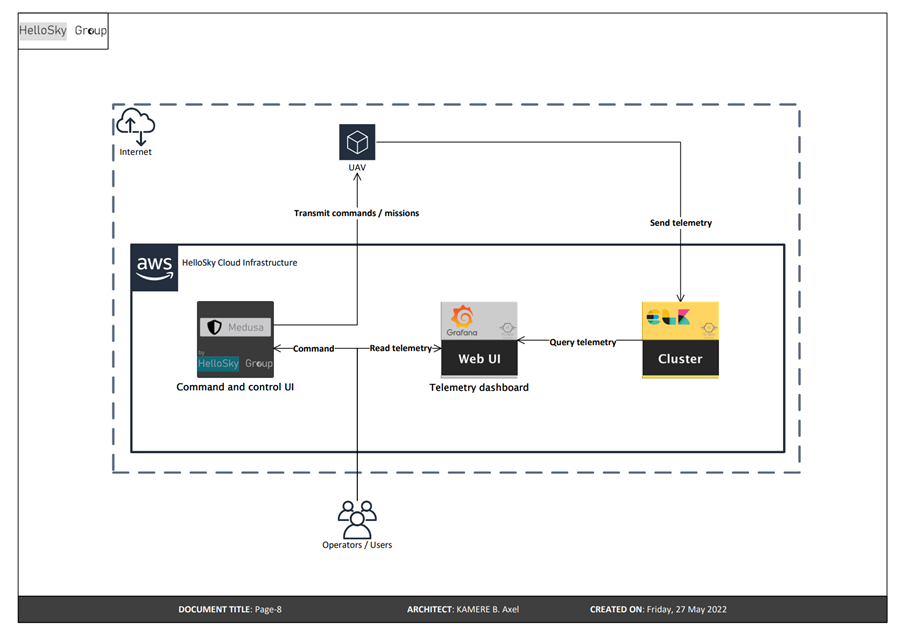
\includegraphics[width=1\linewidth]{UAS HHLD.png}
    \caption{Proposed system high-high-level design.}
    \label{fig:uas-hhld}
    \source{Own work. Designed with Microsoft Visio. Refer to \ref{subsec:ms-visio}.}
\end{figure}


\section{Related work}
\label{sec:related-work}

UAVs and UASs in general is a field that has undergone substantial development through various researches done by scientists, engineers and academicians.

One of the challenges still faced by UAVs, especially in the capability of being able to deploy them in urban areas, is the safety of their operations. Being able to build a UAV with highly effective collision avoidance algorithms is a still a field under active research. And this is one of the main challenges that need to be solved for the world to see robust autonomous UAVs employed widely in communities for various use cases. Pedro et. al have studied on how UAVs can be made more resiliant and safe with the help of artificial intelligence, machine learning and the likes. In their article "Framework for fully autonomous UAVs"~\cite{Pedro2020}, they reviewed the current collision avoidance algorithms for both static and dynamic objects and proposed a conceptual framework to improve more the safety and realiability of UAVs.

<ADD ONE MORE USECASE, CLOUD RELATED??>

%---------------------------------1.1 Problem definition---------------------------------%
\section{Problem definition}
\label{sec:problem-definition}
The cloud technology is an evolving area nowadays due to how agile, efficient, scalable and cost effective it is to deploy resources on the cloud. Many companies all over the world have seen multiple success stories in using cloud services where, for example, General Electric Renewable Energy has managed to achieve a 99.9\% data availability through its move to the cloud\cite{awsgerenewableenergy}.

The use of cloud services is yet to expand even more to other industries like the aerospace industry, especially in the management of unmanned aerial systems (UAS). As the world sees great use of unmanned aerial vehicles (UAVs), more efficient, reliable, scalable and highly available ways of deploying and operating components of the UAS will need to be developed. Building UASs where the UAV compute power can be on the cloud, as well as other components like the command and control centre would play a big part in advancing the unmanned aerial mobility sector. This can help in increasing the range in which UAVs that rely on battery power operate for example, because the UAV would not need to carry heavy compute power to process its generated data like imagery, as everything would be sent to the cloud to be processed. Therefore, the aim of this thesis is to expand on the question below:

\begin{itemize}
    \item How can one take advantage of cloud computing to deploy an unmanned aerial system in a more efficient, scalable and highly available manner?
    \item What advantage is therein running applications on the cloud?
\end{itemize}


%---------------------------------1.2 Use case---------------------------------%
\section{Use case}
\label{sec:use-case}

As UAVs emerge, there will be a need to be able to centrally manage a fleet of UAVs. Depending on the UAV use case, operators might need to also control them at a long distance beyond eyesight. A UAV operates as part of a system comprised of multiple other components that support the operation of a UAV. The main components are a Ground Control System, <RESEARCH ON THE MAIN COMPONENT OF A UAV>. UAVs can either be fully autonomous, fully manual, or semi-autonomous. UAVs can also be employed in various use cases, below are various scenarios in which UAVs can be used <CITE SOURCES OF THE BELOW USE CASES>
\begin{itemize}
    % https://enterprise-insights.dji.com/blog/drones-in-agriculture#:~:text=Agriculture%20drones%20can%20be%20used,quality%2C%20and%20increased%20yield%20rate.
    \item Agricuture.
    \item Facility inspection.
    \item Terrain mapping.
    \item Shipping and delivery.
    \item Search and rescue.
    \item Law enforcement.
    \item Military reconnaissance / Surveillance.
\end{itemize}

For a UAV to perform any of the above, it needs to meet certain criteria, a UAV should:
\begin{itemize}
    \item Have onboard computer to process mission commands on the fly.
    \item Have onboard key components like,
          \begin{itemize}
              \item Sensors, depending on the mission.
              \item Cameras.
              \item Battery.
              \item LTE modules or Satnav modules to allow communication with ground control.
          \end{itemize}
    \item Have LTE or Satellite communication to enable the UAV to set up a datalink with the ground control. The UAV would have to send data such as
          \begin{itemize}
              \item	Ground speed.
              \item	Altitude.
              \item	Battery levels.
              \item	Yaw.
              \item	Location.
              \item	Direction.
              \item	Sensor data.
              \item	Send the data frequently for real-time or near real-time communication.
              \item	Be able to react and if necessary, take evasive maneuvers when:
                    \begin{itemize}
                        \item On collision course.
                        \item The batteries are low on power.
                        \item Out of connectivity range.
                    \end{itemize}
          \end{itemize}
\end{itemize}

%---------------------------------About HelloSky Group---------------------------------%
\section{About HelloSky group}
\label{sec:about-hellosky-group}

Across this thesis, there will be mentions of the name "HelloSky group". Several designs built for the project as well as source codes all have mentions of HelloSky group or hsg in abbreviations.

HelloSky group is a name that I came up with to label my work done and future developments that will be made on this project and many other related projects that will be built in the future. It is mainly done like so to improve motivation to keep working on the project, be it now or in the future. Figure \ref{fig:hs-group-logos} shows the HelloSky group logos that will be seen across various figures and source codes throughout the thesis project.

\begin{figure}[!htbp]
    \centering
    \begin{subfigure}{0.4\textwidth}
        
\includegraphics[width=\linewidth]{hs_group_wide_500x200.png}
        \caption{Colored 500 x 200.}
        \label{fig:hs-group-wide-500x200}
    \end{subfigure}
    \hspace*{\fill}
    \begin{subfigure}{0.4\textwidth}
        
\includegraphics[width=\linewidth]{hs_group_wide_dark_500x200.png}
        \caption{Black and white 500 x 200.}
        \label{fig:hs-group-wide-dark-500x200}
    \end{subfigure}
    \caption{HelloSky group logos.}
    \label{fig:hs-group-logos}
    \source{Own work. Designed with Affinity Designer. Refer to \ref{subsec:affinity-designer}.}
\end{figure}


\nomenclature[z-UAV]{UAV}{Unmanned Aerial Vehicle}
\nomenclature[z-UAS]{UAS}{Unmanned Aerial System}
\nomenclature[z-GCS]{GCS}{Ground Control Station}
\nomenclature[z-LTE]{LTE}{Long Term Evoluton (Telecommunication)}
\nomenclature[z-DJI]{DJI}{Da-Jiang Innovations}
\nomenclature[z-AWS]{AWS}{Amazon Web Services}
\nomenclature[z-HLD]{HLD}{High-Level Design}
\nomenclature[z-HHLD]{HHLD}{High-High-Level Design}